\documentclass{article}[10pt]
\usepackage{multicol, enumerate, enumitem, hyperref, color, soul, setspace, parskip, fancyhdr, amssymb, amsthm, amsmath, bbm, latexsym, units, mathtools}
\everymath{\displaystyle}
\usepackage[headsep=0.5cm,headheight=0cm, left=1 in,right= 1 in,top= 1 in,bottom= 1 in]{geometry}

\begin{document}
This is the Answer Key for Module 5 Version B.

21. What is the domain of the function below?
$$ f(x) = \sqrt[4]{-6 x - 3} $$ 
The solution is $ (-\infty, -0.500000] $ 

\begin{enumerate}[label=\Alph*.] 
\item $ (-\infty, a], \text{where } a \in [-6, -1] $ 

 This distractor corresponds to the pivot -2.000000. 
\item $ [a, \infty), \text{where } a \in [-0.9, 0.3] $ 

 This distractor corresponds to reversing the direction of the domain. 
\item $ (-\infty, a], \text{ where } a \in [-1, 1] $ 

 * This is the correct option. 
\item $ [a, \infty), \text{where } a \in [-4, -0.7] $ 

 This distractor corresponds to reversing the direction of the domain AND the pivot -2.000000. 
\item $ (-\infty, \infty) $ 

 This distractor corresponds to the radical having an odd power. 
\end{enumerate} 
 
Remember that we cannot take the even root of a negative number - this is why the domain is only sometimes restricted! If we have an even root, we solve $-6 x - 3 \geq 0$. Since this is an inequality, remember to flip the inequality if we divide by a negative number.

-----------------------------------------------

22. Choose the equation of the function graphed below.
$$ \text{Graph of the function } f(x) = \sqrt[3]{x - 14} + 5 $$ 
\begin{center}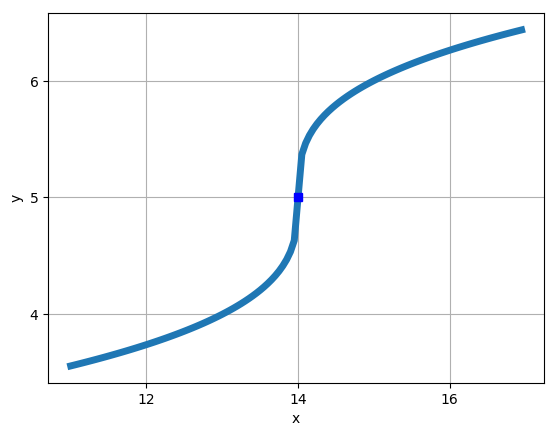
\includegraphics[scale=0.5]{../Figures/question22B.png}\end{center}The solution is $ \sqrt[3]{x - 14} + 5 $ 

\begin{enumerate}[label=\Alph*.] 
\item $ \sqrt[3]{x - 14} + 5 $ 

 This is the correct option. 
\item $ - \sqrt[3]{x + 14} + 5 $ 

 Corresponds to switching the coefficient AND switching the $x$-value of the vertex. 
\item $ \sqrt[3]{x + 14} + 5 $ 

 Corresponds to the correct coefficient and switching the $x$-value of the vertex. 
\item $ - \sqrt[3]{x - 14} + 5 $ 

 Corresponds to switching the coefficient and having the correct vertex. 
\end{enumerate} 
 
General Comments: Remember that the general form of a radical equation is $ f(x) = a \sqrt[b]{x - h} + k$, where $a$ is the leading coefficient (and in this case, we assume is either $1$ or $-1$), $b$ is the root degree (in this case, either $2$ or $3$), and $(h, k)$ is the vertex.

-----------------------------------------------

23. Choose the graph of the equation below.
$$ \sqrt{x + 10} + 7 $$ 
The solution is  
\begin{center}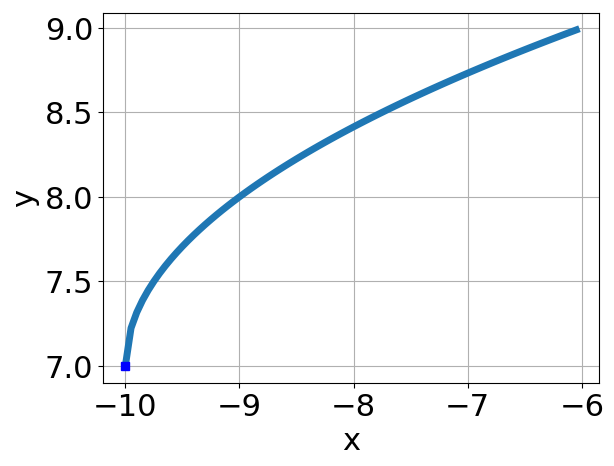
\includegraphics[scale=0.5]{../Figures/question23BD.png}\end{center}\begin{enumerate}[label=\Alph*.] 
\item This is the correct option. 
\begin{center}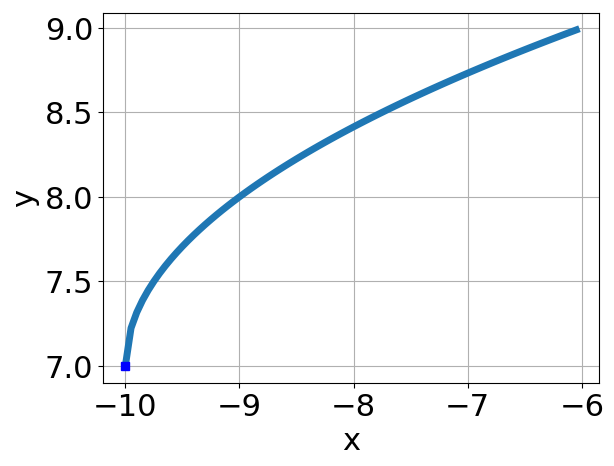
\includegraphics[scale=0.5]{../Figures/question23BD.png}\end{center} 
 
\item Corresponds to switching the coefficient and having the correct vertex. 
\begin{center}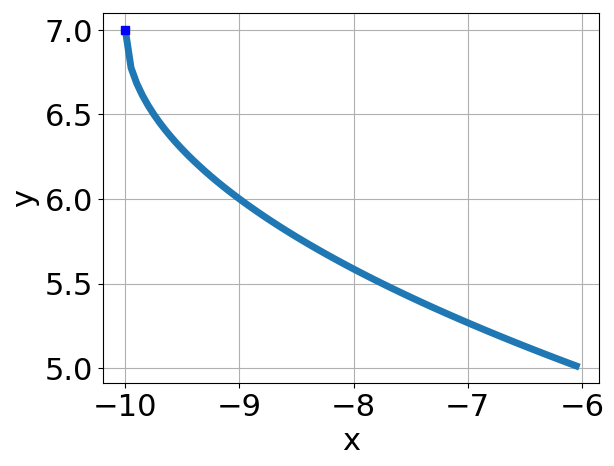
\includegraphics[scale=0.5]{../Figures/question23BC.png}\end{center} 
 
\item Corresponds to the correct coefficient and switching the $x$-value of the vertex. 
\begin{center}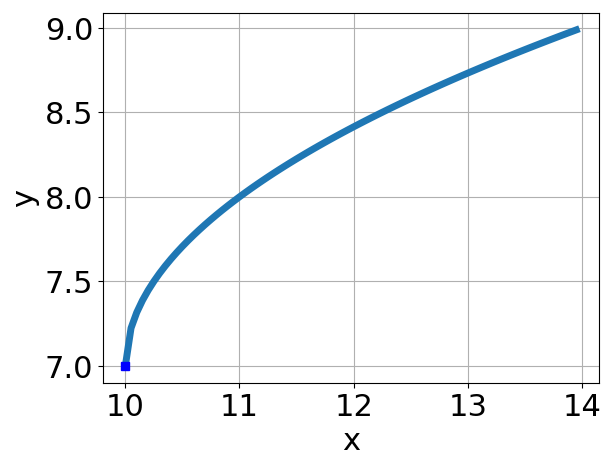
\includegraphics[scale=0.5]{../Figures/question23BB.png}\end{center} 
 
\item Corresponds to switching the coefficient AND switching the $x$-value of the vertex. 
\begin{center}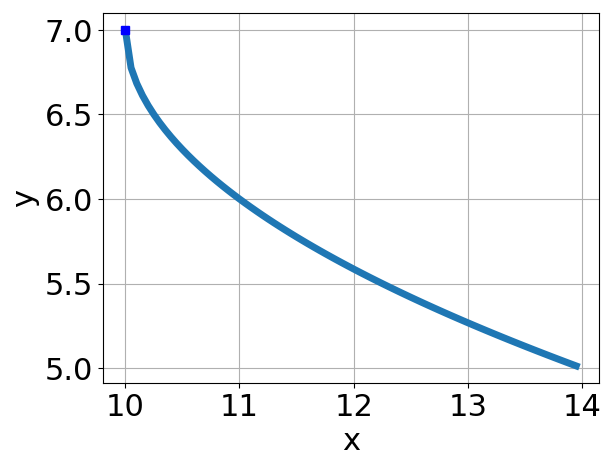
\includegraphics[scale=0.5]{../Figures/question23BA.png}\end{center} 
 
\end{enumerate} 
 
General Comments: Remember that the general form of a radical equation is $ f(x) = a \sqrt[b]{x - h} + k$, where $a$ is the leading coefficient (and in this case, we assume is either $1$ or $-1$), $b$ is the root degree (in this case, either $2$ or $3$), and $(h, k)$ is the vertex.

-----------------------------------------------

24. Solve the radical equation below. Then, choose the interval(s) that the solution(s) belongs to.
$$ \sqrt{-8 x - 8} - \sqrt{-4 x - 7} = 0 $$ 
The solution is $ \text{All solutions lead to invalid or complex values in the equation.} $ 

\begin{enumerate}[label=\Alph*.] 
\item $ x \in [-0.4,0.07] $ 

  
\item $ x_1 \in [-0.4, 0.07] \text{ and } x_2 \in [-2,7] $ 

  
\item $ x \in [-0.23,0.26] $ 

  
\item $ \text{All solutions lead to invalid or complex values in the equation.} $ 

 * This is the correct option. 
\item $ x_1 \in [-0.4, 0.07] \text{ and } x_2 \in [-8,-2] $ 

  
\end{enumerate} 
 
General Comments: Distractors are different based on the number of solutions. For example, if the question is designed to have 0 options, then the distractors are solving the equation and not checking that the solution leads to complex numbers (because plugging them in makes the value under the square root negative). Remember that after solving, we need to make sure our solution does not make the original equation take the square root of a negative number!

-----------------------------------------------


\end{document}
